\documentclass[a4paper,10pt]{article}
\usepackage[utf8]{inputenc}
\usepackage[top=2.5cm, bottom=2.5cm, left=2.5cm, right=2.5cm]{geometry}
\usepackage[english]{babel}
\usepackage{graphicx}
\usepackage{listings}
\usepackage[final]{pdfpages} 


% Title Page
\title{Université Libre de Bruxelles \\
INFO-F405 - Computer Security \\
Synchronized File Exchanger}
\author{Groupe 8: \\
Csori Pinto Constanza, Dauphin Guillaume, Deng Rhenzi, Picard Simon}

\begin{document}
\maketitle
\clearpage
\tableofcontents
\clearpage

\section{Introduction}
The prupose of the project is to implement a secure synchronized file exchanger between two computers with the possibility to send or receive a file. In this project we implemented a custom protocol and we used AES and RSA algorithm to encrypt and decrypt data in order to securely send informations. We also use SHA3 hash generate signature and thus verify the identity of the correspondant.


\section{Implementation}
The project is coded in Java.\\
The generation of the key was not to be handle by the project but using openssl.\\
Here are the commands that lead to the required files by the project :
\begin{verbatim}
openssl req -x509 -newkey rsa:2048 -keyout private_key.pem -out public_certificate.pem -days 365
openssl pkcs8 -topk8 -nocrypt -in private_key.pem -inform PEM -out private_key.der -outform DER
openssl x509 -in public_certificate.pem -inform PEM –out public_certificate.der -outform DER
\end{verbatim}
First we generate the private key and the public certificate and the we convert them to DER files that Java can read.\\
\\
AES and RSA implementation were handle by the Java native library javax.crypto.\\
SHA3 implementation were found on the internet.\\
RSA signature with SHA3 was not implemented so it is done as follow : generate SHA3 hash and then encrypt it with private key.\\
The verification wass to hash the same data, decrypt the signature usign the public key and compare the hashes.\\
\\
The GUI was done using SWING.

\section{Code description}

There is two possible action send or receive a file. The receiver is the server and the sender is the client, once the socket are opened the protocol can begin. First the sender, called Alice, send his public certificate and the receiver, called Bob, do the same, after that the Alice generate a nonce by concatenating a 32 bits random number and a timestamp. Then Alice send a session key wich is a random 128 bits number prefixed by his IP and Bob's IP. This message is encrypted in RSA using Bob's public key. Once the session key is sent, Alice send the next message which is the file wrapped by the IPs and the nonce is encrypted in AES using the session key. Then Alice send her signature and Bob verify that it is correct usign Alice's public key. Finally Bob sent a hash to Alice as an acknowledge.


\section{Threat model}


\subsection{Information document}
\fbox{	
	\begin{minipage}{0.9\textwidth}
	\textbf{Step of the development : }Version 1.0\\ 
	\textbf{Director :}  Csori Pinto Constanza, Dauphin Guillaume, Deng Rhenzi, Picard Simon \\
	\textbf{Participants :} Csori Pinto Constanza, Dauphin Guillaume, Deng Rhenzi, Picard Simon\\
	\textbf{Reviewer :} Csori Pinto Constanza, Dauphin Guillaume, Deng Rhenzi, Picard Simon\\
	\textbf{Localisation :} ULB\\
	\textbf{Description :} The group of students from ULB has created an application for secure file exchange between two users. The file is encrypted and the system uses a encrypted secure protocol.
	\end{minipage}
}


\subsection{External dependencies}

\fbox{
	\begin{minipage}{0.9\textwidth}
	\textbf{ID : } 1\\ 
	\textbf{Description : } The software runs on two computers. Because the code is in Java, it can be easily ported on smartphones or tablet.\\
	\newline
	\textbf{ID : } 2\\ 
	\textbf{Description : } Both computers are connected to each other. The system works with cable connection or wifi.\\
	\newline
	\textbf{ID : } 3\\ 
	\textbf{Description : } There is a firewall on each computer.\\
	\newline
	\textbf{ID : } 4\\ 
	\textbf{Description : } The OS on the computers can be any OS.\\
	\end{minipage}
}
\subsection{Implementation assumptions}

\fbox{
	\begin{minipage}{0.9\textwidth}
	\textbf{ID : } 1\\ 
	\textbf{Description : } The random numbers are considered as random even if they're not perfectly random.\\
	\newline
	\textbf{ID : } 2\\ 
	\textbf{Description : } The implementations of hashing and encryption algorithms must be secure and they must never leak sensitive data through buffer overflows, data in shared memory, etc.\\
	\newline
	\textbf{ID : } 3\\ 
	\textbf{Description : } Java handle de sockets gestion therefor their implementation must be secure.\\
	\end{minipage}
}
\subsection{External security notes}

\fbox{
	\begin{minipage}{0.9\textwidth}
	\textbf{ID : } 1\\ 
	\textbf{Description : } Firewall must be set up with open port for the socket in java.\\
	\newline
	\textbf{ID : } 2\\ 
	\textbf{Description : } The sender and the receiver must provide a private key to the program, they should not share this key.\\
	\end{minipage}
}
\subsection{Internal security notes}

\fbox{
	\begin{minipage}{0.9\textwidth}
	\textbf{ID : } 1\\ 
	\textbf{Description : } OpenSSL is used to generate RSA key pairs. Thus we rely on OpenSSL not leaking sensitive data (e.g. it must not make keys accessible through some system hack), and OpenSSL must generate correct and secure RSA certificates.\\
	\newline
	\textbf{ID : } 2\\ 
	\textbf{Description : } The server and client programs are implemented in Java, using libraries that provide AES and RSA implementations\\
	\end{minipage}
}
\subsection{Levels of trust}

\fbox{
	\begin{minipage}{0.9\textwidth}
	\textbf{ID : } 1\\ 
	\textbf{Name : } Application\\
	\textbf{Description : } The application itself communicate to the same application on the second computer.\\
	\newline
	\textbf{ID : } 2\\ 
	\textbf{Name : } Internet\\
	\textbf{Description : } Online application and connection to the computer. No permission on the application.\\
	\newline
	\textbf{ID : } 3\\ 
	\textbf{Name : } Local Network\\
	\textbf{Description : } User or application on the local Network. No permission on the application.\\
	\newline
	\textbf{ID : } 4\\ 
	\textbf{Name : } Bluetooth User\\
	\textbf{Description : } User or application using bluetooth near the computer of the sender or the receiver. No permission on the application.\\
	\newline
	\textbf{ID : } 5\\ 
	\textbf{Name : } User\\
	\textbf{Description : } The User of the application (sender or receiver).\\
	\end{minipage}
}
\subsection{Entry points}

\fbox{
	\begin{minipage}{0.9\textwidth}
	\textbf{ID : } 1\\ 
	\textbf{Name : } Ethernet port\\
	\textbf{Description : } Both computers are connected via a ethernet cable to each other.\\
	\textbf{Level of trust : } (1) Application\\
	\newline
	\textbf{ID : } 2\\ 
	\textbf{Name : } Wifi\\
	\textbf{Description : } Both computers are connected via wifi to each other.\\
	\textbf{Level of trust : } (1) Application, (2) Internet, (3) Local Network\\
	\newline
	\textbf{ID : } 3\\ 
	\textbf{Name : } Bluetooth\\
	\textbf{Description : } Both computers are connected via bluetooth to each other.\\
	\textbf{Level of trust : } (1) Application, (4) Bluetooth User\\
	\newline
	\textbf{ID : } 4\\ 
	\textbf{Name : } File\\
	\textbf{Description : } The application is used to exchange files. At a given moment, the user must give a file to the application.\\
	\textbf{Level of trust : } (5) User\\
	\newline
	\textbf{ID : } 5\\ 
	\textbf{Name : } Keys\\
	\textbf{Description : } The keys are used for the encryption. A code injection can come through that + buffer overflow.\\
	\textbf{Level of trust : } (1) Application\\
	\end{minipage}
}
\subsection{Assets}

\fbox{
	\begin{minipage}{0.9\textwidth}
	\textbf{ID : } 1\\ 
	\textbf{Name : } IP Address\\
	\textbf{Description : } The IP adress is used as identifier for the users in the program. It will be encrypted during the process.\\
	\textbf{Level of trust : } (1) Application, (5) User\\
	\newline
	\textbf{ID : } 2\\ 
	\textbf{Name : } Session key\\
	\textbf{Description : } The session key is used to encrypt the file that Alice wants to send to Bob.\\
	\textbf{Level of trust : } (1) Application, (5) User\\
	\newline
	\textbf{ID : } 3\\ 
	\textbf{Name : } Private key\\
	\textbf{Description : } Used to create the signature.\\
	\textbf{Level of trust : } (1) Application, (5) User\\
	\newline
	\textbf{ID : } 4\\ 
	\textbf{Name : } Signature\\
	\textbf{Description : } The signature is used to confirm the personnality of the sender.\\
	\textbf{Level of trust : } (1) Application, (5) User\\
	\newline
	\textbf{ID : } 5\\ 
	\textbf{Name : } File\\
	\textbf{Description : } The file sent by the user.\\
	\textbf{Level of trust : } (1) Application, (5) User\\
	\end{minipage}
}

\section{Model analysis}

\subsection{Data flow diagram}
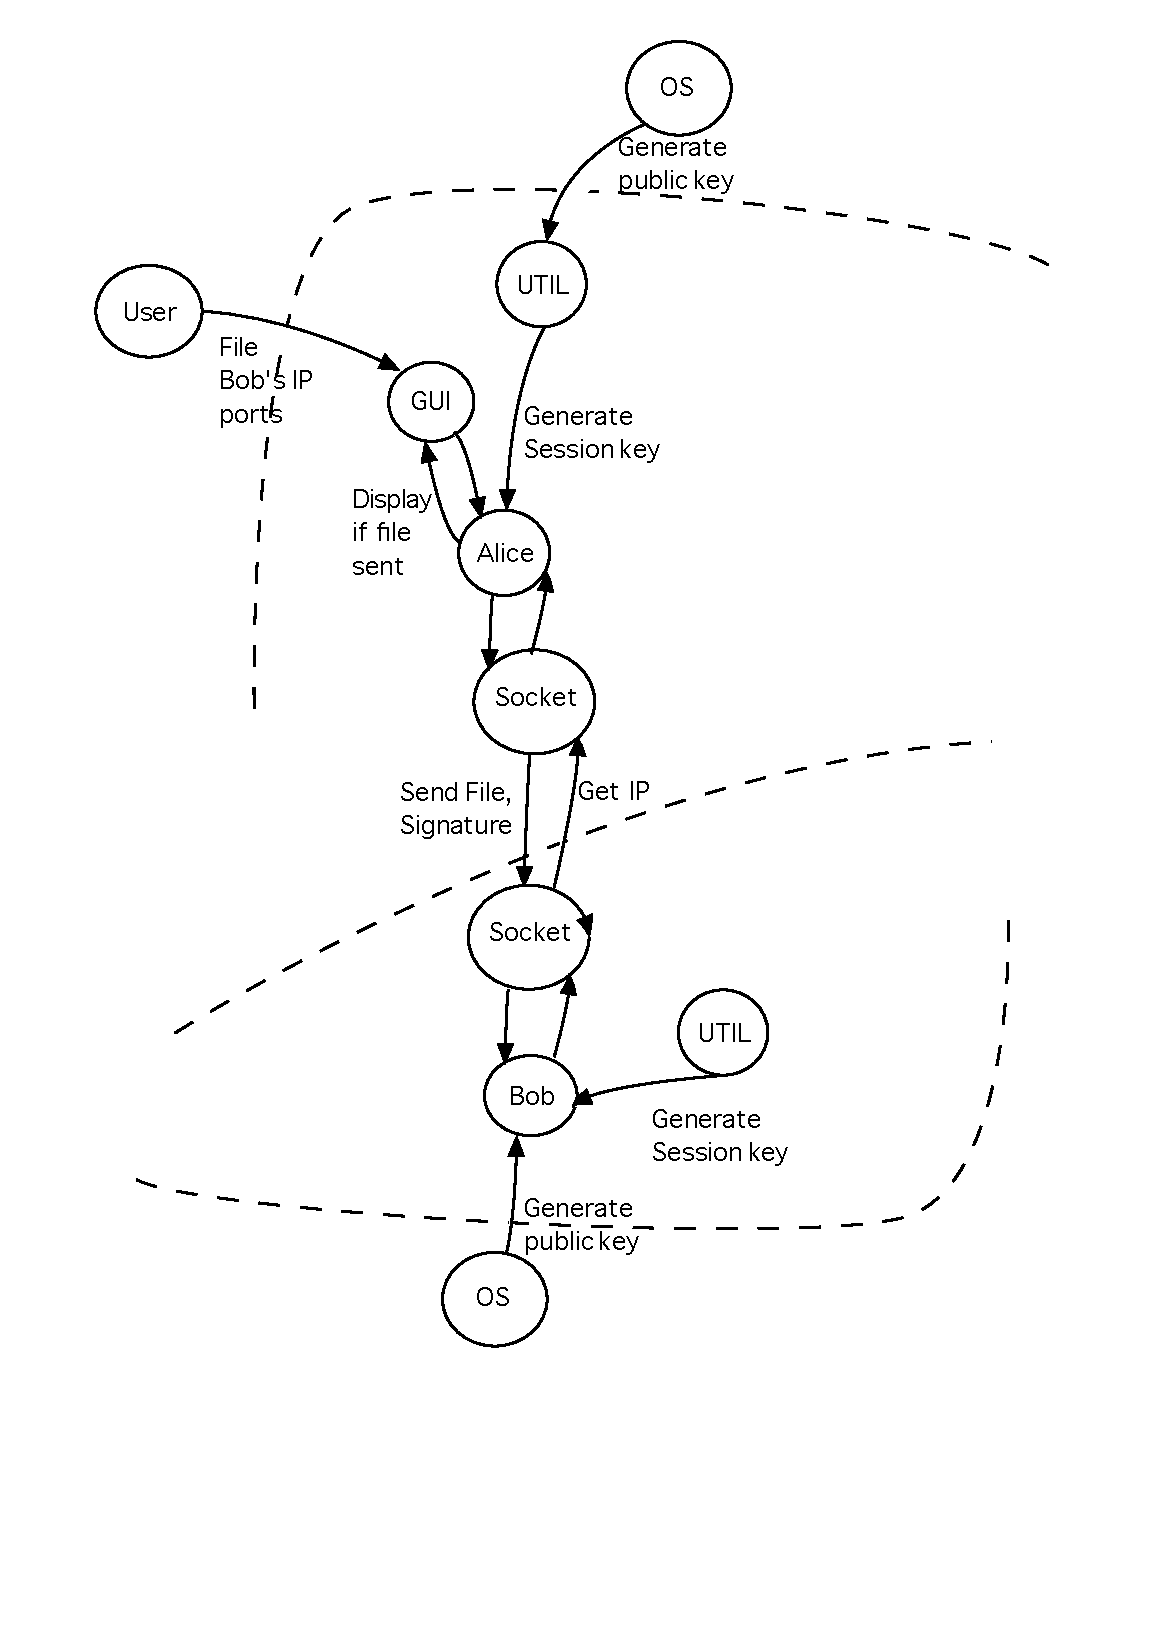
\includepdf[pages=1-1]{threat.pdf}

\subsection{Potential threats}

\section{Conclusion}
The goal of the project was to send a file over the network in a secure way, using AES and RSA encryption and SHA3 hash, following a given protocol. First the sender distribute an AES key that is send encrypted by RSA and then the file is encrypted using AES. The design of the exchange prevent anyone but the receiver to decrypt the file if someone is able to intercept the messages.\\
Symmetric encryption and fecryption is often mor efficent and fits better for larger volume of date than assymetrics ciphers but a shared key is mandotory, so first a random session key is sent on the network encrypted using assymetric encryptoin, RSA, and then, for the large message, the file, it is encrypted using symmetric encryption, AES.

\end{document}          
